% *** Authors should verify (and, if needed, correct) their LaTeX system  ***
% *** with the testflow diagnostic prior to trusting their LaTeX platform ***
% *** with production work. IEEE's font choices can trigger bugs that do  ***
% *** not appear when using other class files.                            ***
% The testflow support page is at:
% http://www.michaelshell.org/tex/testflow/


%%*************************************************************************
%% Legal Notice:
%% This code is offered as-is without any warranty either expressed or
%% implied; without even the implied warranty of MERCHANTABILITY or
%% FITNESS FOR A PARTICULAR PURPOSE!
%% User assumes all risk.
%% In no event shall IEEE or any contributor to this code be liable for
%% any damages or losses, including, but not limited to, incidental,
%% consequential, or any other damages, resulting from the use or misuse
%% of any information contained here.
%%
%% All comments are the opinions of their respective authors and are not
%% necessarily endorsed by the IEEE.
%%
%% This work is distributed under the LaTeX Project Public License (LPPL)
%% ( http://www.latex-project.org/ ) version 1.3, and may be freely used,
%% distributed and modified. A copy of the LPPL, version 1.3, is included
%% in the base LaTeX documentation of all distributions of LaTeX released
%% 2003/12/01 or later.
%% Retain all contribution notices and credits.
%% ** Modified files should be clearly indicated as such, including  **
%% ** renaming them and changing author support contact information. **
%%
%% File list of work: IEEEtran.cls, New_IEEEtran_how-to.pdf, bare_jrnl_new_sample4.tex,
%%*************************************************************************
\PassOptionsToPackage{unicode}{hyperref}
\PassOptionsToPackage{hyphens}{url}
\PassOptionsToPackage{dvipsnames,svgnames,x11names}{xcolor}
% Note that the a4paper option is mainly intended so that authors in
% countries using A4 can easily print to A4 and see how their papers will
% look in print - the typesetting of the document will not typically be
% affected with changes in paper size (but the bottom and side margins will).
% Use the testflow package mentioned above to verify correct handling of
% both paper sizes by the user's LaTeX system.
%
% Also note that the "draftcls" or "draftclsnofoot", not "draft", option
% should be used if it is desired that the figures are to be displayed in
% draft mode.
%
\documentclass[
  journal,
]{IEEEtran}%
% If IEEEtran.cls has not been installed into the LaTeX system files,
% manually specify the path to it like:
% \documentclass[journal]{../sty/IEEEtran}
\usepackage[cmex10]{amsmath}
\usepackage{amssymb}
\usepackage{iftex}
\ifPDFTeX
  \usepackage[T1]{fontenc}
  \usepackage[utf8]{inputenc}
  \usepackage{textcomp} % provide euro and other symbols
\else % if luatex or xetex
  \usepackage{unicode-math} % this also loads fontspec
  \defaultfontfeatures{Scale=MatchLowercase}
  \defaultfontfeatures[\rmfamily]{Ligatures=TeX,Scale=1}
\fi
%\usepackage{lmodern}
\ifPDFTeX\else
\fi
% Use upquote if available, for straight quotes in verbatim environments
\IfFileExists{upquote.sty}{\usepackage{upquote}}{}
\IfFileExists{microtype.sty}{% use microtype if available
  \usepackage[]{microtype}
  \UseMicrotypeSet[protrusion]{basicmath} % disable protrusion for tt fonts
}{}
\makeatletter
\parindent    1.0em
\ifCLASSOPTIONcompsoc
  \parindent    1.5em
\fi
\makeatother
\usepackage{xcolor}
\setlength{\emergencystretch}{3em} % prevent overfull lines

\setcounter{secnumdepth}{5}
% Make \paragraph and \subparagraph free-standing
\ifx\paragraph\undefined\else
  \let\oldparagraph\paragraph
  \renewcommand{\paragraph}[1]{\oldparagraph{#1}\mbox{}}
\fi
\ifx\subparagraph\undefined\else
  \let\oldsubparagraph\subparagraph
  \renewcommand{\subparagraph}[1]{\oldsubparagraph{#1}\mbox{}}
\fi


\providecommand{\tightlist}{%
  \setlength{\itemsep}{0pt}\setlength{\parskip}{0pt}}\usepackage{longtable,booktabs,array}
\usepackage{calc} % for calculating minipage widths
% Correct order of tables after \paragraph or \subparagraph
\usepackage{etoolbox}
\makeatletter
\patchcmd\longtable{\par}{\if@noskipsec\mbox{}\fi\par}{}{}
\makeatother
% Allow footnotes in longtable head/foot
\IfFileExists{footnotehyper.sty}{\usepackage{footnotehyper}}{\usepackage{footnote}}
\makesavenoteenv{longtable}
\usepackage{graphicx}
\makeatletter
\def\maxwidth{\ifdim\Gin@nat@width>\linewidth\linewidth\else\Gin@nat@width\fi}
\def\maxheight{\ifdim\Gin@nat@height>\textheight\textheight\else\Gin@nat@height\fi}
\makeatother
% Scale images if necessary, so that they will not overflow the page
% margins by default, and it is still possible to overwrite the defaults
% using explicit options in \includegraphics[width, height, ...]{}
\setkeys{Gin}{width=\maxwidth,height=\maxheight,keepaspectratio}
% Set default figure placement to htbp
\makeatletter
\def\fps@figure{htbp}
\makeatother

\usepackage{physics}
\usepackage[version=3]{mhchem}
\usepackage{orcidlink}
\usepackage{float}
\floatplacement{table}{htb}
\makeatletter
\makeatother
\makeatletter
\makeatother
\makeatletter
\@ifpackageloaded{caption}{}{\usepackage{caption}}
\AtBeginDocument{%
\ifdefined\contentsname
  \renewcommand*\contentsname{Table of contents}
\else
  \newcommand\contentsname{Table of contents}
\fi
\ifdefined\listfigurename
  \renewcommand*\listfigurename{List of Figures}
\else
  \newcommand\listfigurename{List of Figures}
\fi
\ifdefined\listtablename
  \renewcommand*\listtablename{List of Tables}
\else
  \newcommand\listtablename{List of Tables}
\fi
\ifdefined\figurename
  \renewcommand*\figurename{Fig.}
\else
  \newcommand\figurename{Fig.}
\fi
\ifdefined\tablename
  \renewcommand*\tablename{Table}
\else
  \newcommand\tablename{Table}
\fi
}
\@ifpackageloaded{float}{}{\usepackage{float}}
\floatstyle{ruled}
\@ifundefined{c@chapter}{\newfloat{codelisting}{h}{lop}}{\newfloat{codelisting}{h}{lop}[chapter]}
\floatname{codelisting}{Listing}
\newcommand*\listoflistings{\listof{codelisting}{List of Listings}}
\makeatother
\makeatletter
\@ifpackageloaded{caption}{}{\usepackage{caption}}
\@ifpackageloaded{subcaption}{}{\usepackage{subcaption}}
\makeatother
\makeatletter
\@ifpackageloaded{tcolorbox}{}{\usepackage[skins,breakable]{tcolorbox}}
\makeatother
\makeatletter
\@ifundefined{shadecolor}{\definecolor{shadecolor}{rgb}{.97, .97, .97}}
\makeatother
\makeatletter
\makeatother
\makeatletter
\makeatother
\usepackage[skip=2pt,font=footnotesize]{caption}
%\captionsetup{format=myformat}
\ifLuaTeX
  \usepackage{selnolig}  % disable illegal ligatures
\fi
\IfFileExists{bookmark.sty}{\usepackage{bookmark}}{\usepackage{hyperref}}
\IfFileExists{xurl.sty}{\usepackage{xurl}}{} % add URL line breaks if available
\urlstyle{same} % disable monospaced font for URLs
\hypersetup{
  pdftitle={Detecting computing-enabled interdisciplinary domains using the MIDFIELD data set},
  pdfauthor={Tim Ransom; Randi Sims; Stephanie Damas},
  pdfkeywords={Undergraduate Education, Curriculum and Course
Development},
  colorlinks=true,
  linkcolor={blue},
  filecolor={Maroon},
  citecolor={Blue},
  urlcolor={Blue},
  pdfcreator={LaTeX via pandoc}}

% *** Do not adjust lengths that control margins, column widths, etc. ***
% *** Do not use packages that alter fonts (such as pslatex).         ***
% There should be no need to do such things with IEEEtran.cls V1.6 and later.
% (Unless specifically asked to do so by the journal or conference you plan
% to submit to, of course. )


% correct bad hyphenation here
\hyphenation{op-tical net-works semi-conduc-tor}

%
% paper title
% can use linebreaks \\ within to get better formatting as desired
% Do not put math or special symbols in the title.
% paper title
% can use linebreaks \\ within to get better formatting as desired
% Do not put math or special symbols in the title.
\title{Detecting computing-enabled interdisciplinary domains using the
MIDFIELD data set}

\author{
Tim Ransom\orcidlink{0000-0003-0357-5427},~Randi
Sims\orcidlink{0000-0003-0357-5427}
and~Stephanie Damas\orcidlink{0000-0001-5397-7577}%
\thanks{Tim Ransom is with Engineering and Science Education, Clemson
University, Clemson, 29634 United States of America%
 e-mail: tsranso@clemson.edu}
%by-author.affiliations
\thanks{Randi Sims is with Engineering and Science Education, Clemson
University, Clemson, 29634 United States of America%
 e-mail: rsims@clemson.edu}
%by-author.affiliations
\thanks{Stephanie Damas is with Engineering and Science
Education, Clemson University, Clemson, 29634 United States of America%
 e-mail: damas@clemson.edu}
%by-author.affiliations
}
\begin{document}

% The paper headers

% use for special paper notices

% make the title area
\maketitle

% As a general rule, do not put math, special symbols or citations
% in the abstract or keywords.
\begin{abstract}
This work-in-progress research paper presents initial results from a
curriculum analysis of computing-enabled interdisciplinary STEM
programs.

Interdisciplinary curriculum development has been supported through
integrating computing courses for decades. These specialized programs
offer a targeted approach to solving complex issues and act as a point
of attraction for students to enroll in one University over another.
These interdisciplinary programs' curricula often include courses from
their respective ``parent'' fields. For example, a bioinformatics
curriculum can consist of courses from both computer science departments
and biology departments. Specialized courses are often also created in
the ``child'' field to meet the needs of the interdisciplinary students
as well.

The Multiple-Institution Database for Investigating Engineering
Longitudinal Development (MIDFIELD) project has collected complete
course records of every student's path toward a degree from eighteen
Universities across the United States of America. This data allows us to
construct sets of courses that students choose to complete to fulfill
their institution's requirements for graduation. We interpret this set
of courses as representing the knowledge, skills, and abilities (KSAs)
of the students who graduate with a given degree, which we use as our
theoretical framework.

This work analyses the robust MIDFIELD data set to identify overlaps
between interdisciplinary degree course requirements and their
``parent'' degree course requirements. The set of courses shared between
curricula can indicate to curriculum designers the set of classes that
other institutions have deemed sufficiently relevant to include and the
courses offered through different departments. Identifying specialized
courses is also valuable to evaluate possible efficient plans to create
new departments at institutions where established ``parent'' programs
are already present.

This study helps lay the groundwork for promoting computing-enabled
interdisciplinary STEM majors to students. Research has demonstrated how
a diverse team of computing-enabled professionals contributes
significantly to solving complex problems. Implementing
interdisciplinary majors can make computer science programs more
attractive to students with marginalized identities who seek to bridge
the gap between their lived experiences addressed through other STEM
programs and computer science fundamentals. As such, this study aims to
identify fundamental computer science courses that other programs have
or can use computing to extend or create interdisciplinary majors.
\end{abstract}
% Note that keywords are not normally used for peerreview papers.
\begin{IEEEkeywords}
Undergraduate Education, Curriculum and Course Development
\end{IEEEkeywords}

% For peer review papers, you can put extra information on the cover
% page as needed:
% \ifCLASSOPTIONpeerreview
% \begin{center} \bfseries EDICS Category: 3-BBND \end{center}
% \fi
%
% For peerreview papers, this IEEEtran command inserts a page break and
% creates the second title. It will be ignored for other modes.
% \IEEEpeerreviewmaketitle

\ifdefined\Shaded\renewenvironment{Shaded}{\begin{tcolorbox}[frame hidden, breakable, borderline west={3pt}{0pt}{shadecolor}, sharp corners, interior hidden, boxrule=0pt, enhanced]}{\end{tcolorbox}}\fi




% Can use something like this to put references on a page
% by themselves when using endfloat and the captionsoff option.
\ifCLASSOPTIONcaptionsoff
  \newpage
\fi

% trigger a \newpage just before the given reference
% number - used to balance the columns on the last page
% adjust value as needed - may need to be readjusted if
% the document is modified later
%\IEEEtriggeratref{8}
% The "triggered" command can be changed if desired:
%\IEEEtriggercmd{\enlargethispage{-5in}}

% Uncomment when use biblatex with style=ieee
%\renewcommand{\bibfont}{\footnotesize} % for IEEE bibfont size

\pagebreak[3]
\begin{IEEEbiography}[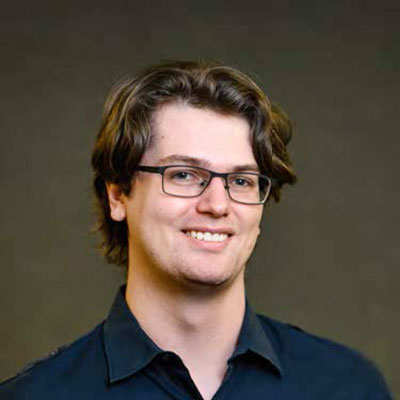
\includegraphics{tim-ransom.jpg}]{Tim Ransom}
Tim Ransom is a PhD candidate in the Clemson University Enigineering and
Science Education department. He studies computer science education
through qualitative and computational methodologies.
\end{IEEEbiography}
\begin{IEEEbiography}[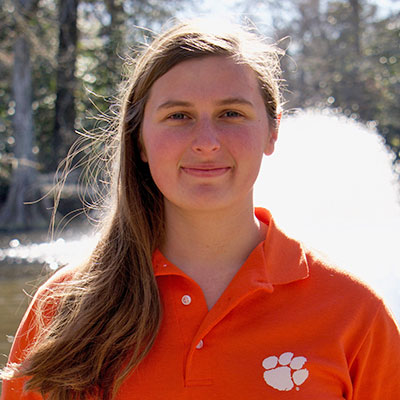
\includegraphics{randi-sims.jpg}]{Randi Sims}
Randi Sims is\ldots{}
\end{IEEEbiography}
\begin{IEEEbiography}[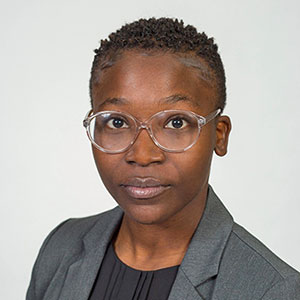
\includegraphics{stephanie-damas.jpg}]{Stephanie
Damas}
Stephanie Damas is\ldots{}
\end{IEEEbiography}
% that's all folks
\end{document}

